% Options for packages loaded elsewhere
\PassOptionsToPackage{unicode}{hyperref}
\PassOptionsToPackage{hyphens}{url}
%
\documentclass[
  8pt,
  ignorenonframetext,
]{beamer}
\usepackage{pgfpages}
\setbeamertemplate{caption}[numbered]
\setbeamertemplate{caption label separator}{: }
\setbeamercolor{caption name}{fg=normal text.fg}
\beamertemplatenavigationsymbolsempty
% Prevent slide breaks in the middle of a paragraph
\widowpenalties 1 10000
\raggedbottom
\setbeamertemplate{part page}{
  \centering
  \begin{beamercolorbox}[sep=16pt,center]{part title}
    \usebeamerfont{part title}\insertpart\par
  \end{beamercolorbox}
}
\setbeamertemplate{section page}{
  \centering
  \begin{beamercolorbox}[sep=12pt,center]{part title}
    \usebeamerfont{section title}\insertsection\par
  \end{beamercolorbox}
}
\setbeamertemplate{subsection page}{
  \centering
  \begin{beamercolorbox}[sep=8pt,center]{part title}
    \usebeamerfont{subsection title}\insertsubsection\par
  \end{beamercolorbox}
}
\AtBeginPart{
  \frame{\partpage}
}
\AtBeginSection{
  \ifbibliography
  \else
    \frame{\sectionpage}
  \fi
}
\AtBeginSubsection{
  \frame{\subsectionpage}
}
\usepackage{amsmath,amssymb}
\usepackage{lmodern}
\usepackage{iftex}
\ifPDFTeX
  \usepackage[T1]{fontenc}
  \usepackage[utf8]{inputenc}
  \usepackage{textcomp} % provide euro and other symbols
\else % if luatex or xetex
  \usepackage{unicode-math}
  \defaultfontfeatures{Scale=MatchLowercase}
  \defaultfontfeatures[\rmfamily]{Ligatures=TeX,Scale=1}
\fi
% Use upquote if available, for straight quotes in verbatim environments
\IfFileExists{upquote.sty}{\usepackage{upquote}}{}
\IfFileExists{microtype.sty}{% use microtype if available
  \usepackage[]{microtype}
  \UseMicrotypeSet[protrusion]{basicmath} % disable protrusion for tt fonts
}{}
\makeatletter
\@ifundefined{KOMAClassName}{% if non-KOMA class
  \IfFileExists{parskip.sty}{%
    \usepackage{parskip}
  }{% else
    \setlength{\parindent}{0pt}
    \setlength{\parskip}{6pt plus 2pt minus 1pt}}
}{% if KOMA class
  \KOMAoptions{parskip=half}}
\makeatother
\usepackage{xcolor}
\newif\ifbibliography
\setlength{\emergencystretch}{3em} % prevent overfull lines
\providecommand{\tightlist}{%
  \setlength{\itemsep}{0pt}\setlength{\parskip}{0pt}}
\setcounter{secnumdepth}{-\maxdimen} % remove section numbering
\newlength{\cslhangindent}
\setlength{\cslhangindent}{1.5em}
\newlength{\csllabelwidth}
\setlength{\csllabelwidth}{3em}
\newlength{\cslentryspacingunit} % times entry-spacing
\setlength{\cslentryspacingunit}{\parskip}
\newenvironment{CSLReferences}[2] % #1 hanging-ident, #2 entry spacing
 {% don't indent paragraphs
  \setlength{\parindent}{0pt}
  % turn on hanging indent if param 1 is 1
  \ifodd #1
  \let\oldpar\par
  \def\par{\hangindent=\cslhangindent\oldpar}
  \fi
  % set entry spacing
  \setlength{\parskip}{#2\cslentryspacingunit}
 }%
 {}
\usepackage{calc}
\newcommand{\CSLBlock}[1]{#1\hfill\break}
\newcommand{\CSLLeftMargin}[1]{\parbox[t]{\csllabelwidth}{#1}}
\newcommand{\CSLRightInline}[1]{\parbox[t]{\linewidth - \csllabelwidth}{#1}\break}
\newcommand{\CSLIndent}[1]{\hspace{\cslhangindent}#1}
% type setting
% ------------------------------------------------------------------------------
\usepackage[german]{babel}     

% fonts
% ------------------------------------------------------------------------------
\usefonttheme{professionalfonts}

% slide title and horizontal line
% ------------------------------------------------------------------------------
\setbeamertemplate{frametitle}{%
    \vskip-30pt \color{black}\large%
    \begin{minipage}[b][23pt]{120mm}%
    \flushleft\insertframetitle%
    \end{minipage}%
}

\setbeamertemplate{headline}										
{
\vskip10pt\hfill\hspace{3.5mm} 										 
\vskip15pt\color{black}\rule{\textwidth}{0.4pt} 					 
}

% slide number
% ---------------------------------------------------------------
\setbeamertemplate{navigation symbols}{}
\setbeamertemplate{footline}
{
\vskip5pt
\vskip2pt
\makebox[123mm]{\hspace{7.5mm}
\hfill Wahrscheinlichkeitstheorie und Frequentistische Inferenz $\vert$ 
\copyright $ $ 2023 Dirk Ostwald CC BY-SA 4.0 $\vert$ 
Folie \insertframenumber}
\vskip4pt
}

% block color scheme
% ------------------------------------------------------------------------------
% colors
\definecolor{white}{RGB}{255,255,255}
\definecolor{grey}{RGB}{235,235,235}
\definecolor{lightgrey}{RGB}{245,245,245}
\definecolor{LightBlue}{RGB}{220,220,255}
\definecolor{darkblue}{RGB}{51, 51, 153}

% definitions and theorems
\setbeamercolor{block title}{fg = black, bg = grey}
\setbeamercolor{block body}{fg = black, bg = lightgrey}

% general line spacing 
% ------------------------------------------------------------------------------
\linespread{1.3}

% local line spacing
% ------------------------------------------------------------------------------
\usepackage{setspace}

% colors
% -----------------------------------------------------------------------------
\usepackage{color}

% justified text
% ------------------------------------------------------------------------------
\usepackage{ragged2e}
\usepackage{etoolbox}
\apptocmd{\frame}{}{\justifying}{}

% bullet point lists
% -----------------------------------------------------------------------------
\setbeamertemplate{itemize item}[circle]
\setbeamertemplate{itemize subitem}[circle]
\setbeamertemplate{itemize subsubitem}[circle]
\setbeamercolor{itemize item}{fg = black}
\setbeamercolor{itemize subitem}{fg = black}
\setbeamercolor{itemize subsubitem}{fg = black}
\setbeamercolor{enumerate item}{fg = black}
\setbeamercolor{enumerate subitem}{fg = black}
\setbeamercolor{enumerate subsubitem}{fg = black}
\setbeamerfont{itemize/enumerate body}{}
\setbeamerfont{itemize/enumerate subbody}{size = \normalsize}
\setbeamerfont{itemize/enumerate subsubbody}{size = \normalsize}

% color links
% ------------------------------------------------------------------------------
\usepackage{hyperref}
\definecolor{urls}{RGB}{204,0,0}
\hypersetup{colorlinks, citecolor = darkblue, urlcolor = urls}


% additional math commands
% ------------------------------------------------------------------------------
\usepackage{bm}                                         
\newcommand{\niton}{\not\owns}
\newcommand{\ups}{\upsilon}
\DeclareMathOperator*{\intinf}{\int_{-\infty}^{\infty}}


% text highlighting
% ------------------------------------------------------------------------------
\usepackage{soul}
\makeatletter
\let\HL\hl
\renewcommand\hl{%
  \let\set@color\beamerorig@set@color
  \let\reset@color\beamerorig@reset@color
  \HL}
\makeatother

% equation highlighting
% -----------------------------------------------------------------------------
\newcommand{\highlight}[2][yellow]{\mathchoice%
  {\colorbox{#1}{$\displaystyle#2$}}%
  {\colorbox{#1}{$\textstyle#2$}}%
  {\colorbox{#1}{$\scriptstyle#2$}}%
  {\colorbox{#1}{$\scriptscriptstyle#2$}}}%

% additional mathematical operators
% ------------------------------------------------------------------------------
\DeclareMathOperator*{\argmax}{arg\,max}
\DeclareMathOperator*{\argmin}{arg\,min}

\ifLuaTeX
  \usepackage{selnolig}  % disable illegal ligatures
\fi
\IfFileExists{bookmark.sty}{\usepackage{bookmark}}{\usepackage{hyperref}}
\IfFileExists{xurl.sty}{\usepackage{xurl}}{} % add URL line breaks if available
\urlstyle{same} % disable monospaced font for URLs
\hypersetup{
  hidelinks,
  pdfcreator={LaTeX via pandoc}}

\author{}
\date{\vspace{-2.5em}}

\begin{document}

\begin{frame}[plain]{}
\protect\hypertarget{section}{}
\center

\begin{center}
\includegraphics[width=0.2\linewidth]{7_Abbildungen/wtfi_7_otto} \end{center}

\vspace{2mm}

\Large

Wahrscheinlichkeitstheorie und Frequentistische Inferenz \vspace{6mm}

\large

BSc Psychologie WiSe 2022/23

\vspace{6mm}
\large

Prof.~Dr.~Dirk Ostwald
\end{frame}

\begin{frame}[plain]{}
\protect\hypertarget{section-1}{}
\vfill
\center
\huge

\textcolor{black}{(7) Ungleichungen und Grenzwerte} \vfill
\end{frame}

\begin{frame}{}
\protect\hypertarget{section-2}{}
\large
\vfill
\setstretch{2.5}

Wahrscheinlichkeitsungleichungen

Erwartungswertungleichungen

Gesetze der Großen Zahl

Zentrale Grenzwertsätze

Selbstkontrollfragen \vfill
\end{frame}

\begin{frame}{}
\protect\hypertarget{section-3}{}
\large
\vfill
\setstretch{2.5}

\textbf{Wahrscheinlichkeitsungleichungen}

Erwartungswertungleichungen

Gesetze der Großen Zahl

Zentrale Grenzwertsätze

Selbstkontrollfragen \vfill
\end{frame}

\begin{frame}{Wahrscheinlichkeitsungleichungen}
\protect\hypertarget{wahrscheinlichkeitsungleichungen}{}
\small
\begin{theorem}[Markov Ungleichung]
\justifying
\normalfont
$\xi$ sei eine Zufallsvariable mit $\mathbb{P}(\xi \ge 0) = 1$. Dann gilt für alle  $x \in \mathbb{R}$, dass
\begin{equation}
\mathbb{P}(\xi \ge x) \le \frac{\mathbb{E}(\xi)}{x}.
\end{equation}
\end{theorem}

Bemerkungen

\begin{itemize}
\tightlist
\item
  Weil \(\mathbb{P}(\xi \ge 0) = 1\) gilt, sagt man auch, dass \(\xi\)
  eine \textit{nicht-negative} Zufallvariable ist.
\item
  Die Ungleichung setzt Überschreitungswahrscheinlichkeiten und
  Erwartungswerte in Bezug.
\item
  Gilt z.B. für eine nichtnegative Zufallsvariable \(\xi\), dass
  \(\mathbb{E}(\xi) = 1\), dann ist
  \(\mathbb{P}(\xi \ge 100) \le 0.01\).
\end{itemize}
\end{frame}

\begin{frame}{Wahrscheinlichkeitsungleichungen}
\protect\hypertarget{wahrscheinlichkeitsungleichungen-1}{}
\footnotesize

\underline{Beweis}

Wir betrachten den Fall einer kontinuierlichen Zufallsvariable \(\xi\)
mit WDF \(p\). Wir halten zunächst fest, dass \begin{equation}
\mathbb{E}(\xi)
= \int_{-\infty}^\infty s \, p(s)\,ds
= \int_0^\infty s \, p(s)\,ds
= \int_0^x s \, p(s)\,ds + \int_x^\infty s \, p(s)\,ds,
\end{equation} weil \(\xi\) nicht-negativ ist. Es folgt dann
\begin{equation}
\mathbb{E}(\xi)
\ge  \int_x^\infty s \, p(s)\,ds
\ge  \int_x^\infty x \, p(s)\,ds
=  x\int_x^\infty  p(s)\,ds
=  x\, \mathbb{P}(\xi \ge x).
\end{equation}

Dabei gilt die erste Ungleichung weil \begin{equation}
\int_{0}^x s \, p(s)\,ds \ge 0 
\end{equation} und die zweite Ungleichung gilt, weil \(x \le \xi\) für
\(\xi \in [x,\infty[\). Es folgt also, dass \begin{equation}
\mathbb{E}(\xi) \ge x\, \mathbb{P}(\xi \ge x)
\Leftrightarrow
\mathbb{P}(\xi \ge x) \le \frac{\mathbb{E}(\xi)}{x}.
\end{equation}

\(\hfill\) \(\Box\)
\end{frame}

\begin{frame}{Wahrscheinlichkeitsungleichungen}
\protect\hypertarget{wahrscheinlichkeitsungleichungen-2}{}
\small

Beispiel (\(\xi \sim G(\alpha,\beta)\)) \vspace{1mm} \small

\begin{itemize}
\item Wir halten ohne Beweis fest, dass für $\xi \sim G(\alpha,\beta)$ gilt, dass $\mathbb{E}(\xi) = \alpha\beta$.
\item Wir betrachten den Fall $\alpha := 5, \beta := 2$, so dass $G(x;5,2) = \chi^2(10)$
\end{itemize}

\begin{center}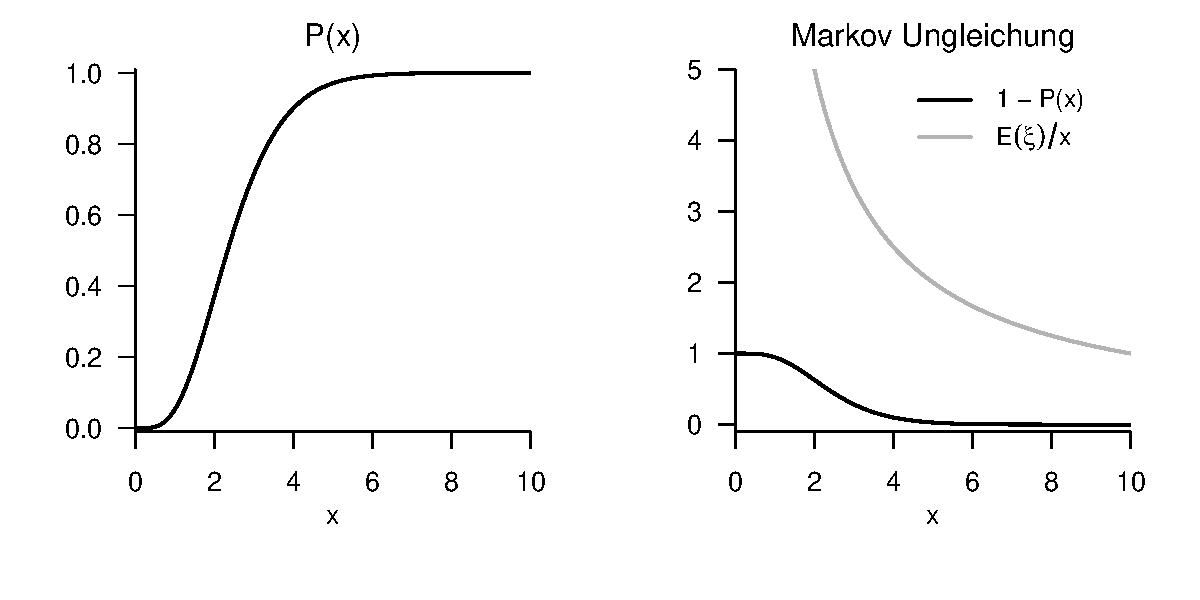
\includegraphics[width=0.95\linewidth]{7_Abbildungen/wtfi_7_markov_ungleichung} \end{center}
\end{frame}

\begin{frame}{Wahrscheinlichkeitsungleichungen}
\protect\hypertarget{wahrscheinlichkeitsungleichungen-3}{}
\small
\begin{theorem}[Chebyshev Ungleichung]
\justifying
\normalfont
Es sei $\xi$ eine Zufallsvariable mit Varianz $\mathbb{V}(\xi)$. Dann gilt für alle $x \in \mathbb{R}$
\begin{equation}
\mathbb{P}(|\xi - \mathbb{E}(\xi)| \ge x) \le \frac{\mathbb{V}(\xi)}{x^2}.
\end{equation}
\end{theorem}

Bemerkungen

\begin{itemize}
\tightlist
\item
  Die Chebyshev Ungleichung setzt Abweichungen vom Erwartungswert in
  Bezug zur Varianz.
\item
  Zum Beispiel gilt \begin{equation}
  \mathbb{P}\left(|\xi - \mathbb{E}(\xi)| \ge 3 \sqrt{\mathbb{V}(\xi)}\right)
  \le  \frac{\mathbb{V}(\xi)}{\left(3 \sqrt{\mathbb{V}(\xi)}\right)^2} =
  \frac{1}{9}.
  \end{equation}
\end{itemize}
\end{frame}

\begin{frame}{Wahrscheinlichkeitsungleichungen}
\protect\hypertarget{wahrscheinlichkeitsungleichungen-4}{}
\footnotesize

\underline{Beweis} \vspace{0.2cm}

Wir halten zunächst fest, dass für \(a,b \in \mathbb{R}\) gilt
\begin{equation}
a^2 \ge b^2 \Leftrightarrow |a| \ge b.
\end{equation} Dazu betrachten wir die folgenden vier möglichen Fälle

\begin{center}
\begin{tabular}{llllll}
$|a| \ge b \mbox{ für } a > 0, b > 0$
& $\Leftrightarrow$
& $\quad a \ge b$
& $\Leftrightarrow$
&
& $\quad\, a^2 \ge b^2$
\\
$|a| \ge b \mbox{ für } a > 0, b < 0$
& $\Leftrightarrow$
& $\quad a \ge b$
& $\Leftrightarrow$
&
& $\quad\, a^2 \ge b^2$
\\
$|a| \ge b \mbox{ für } a < 0, b > 0$
& $\Leftrightarrow$
& $-a \ge b$
& $\Leftrightarrow$
& $(-a)^2 \ge b^2$
& $ = a^2 \ge b^2$
\\
$|a| \ge b \mbox{ für } a < 0, b < 0$
& $\Leftrightarrow$
& $-a \ge b$
& $\Leftrightarrow$
& $(-a)^2 \ge b^2$
& $ = a^2 \ge b^2$
\end{tabular}
\end{center}

Als nächstes definieren wir \(\ups := (\xi - \mathbb{E}(\xi))^2\). Dann
folgt aus der Markov Ungleichung \begin{align}
\begin{split}
\mathbb{P}\left(\ups \ge x^2\right)
& \le \frac{\mathbb{E}(\ups)}{x^2} \\
\Leftrightarrow
\mathbb{P}\left((\xi - \mathbb{E}(\xi))^2 \ge x^2 \right)
& \le \frac{\mathbb{E}\left((\xi - \mathbb{E}(\xi))^2 \right)}{x^2} \\
\Leftrightarrow
\mathbb{P}(|\xi - \mathbb{E}(\xi)| \ge x)
& \le \frac{\mathbb{V}(\xi)}{x^2}.
\end{split}
\end{align} \(\hfill\) \(\Box\)
\end{frame}

\begin{frame}{}
\protect\hypertarget{section-4}{}
\large
\vfill
\setstretch{2.5}

Wahrscheinlichkeitsungleichungen

\textbf{Erwartungswertungleichungen}

Gesetze der Großen Zahl

Zentrale Grenzwertsätze

Selbstkontrollfragen \vfill
\end{frame}

\begin{frame}{Erwartungswertungleichungen}
\protect\hypertarget{erwartungswertungleichungen}{}
\small
\begin{theorem}[Cauchy-Schwarz-Ungleichung]
\normalfont
\justifying
$\xi$ und $\ups$ seien zwei Zufallsvariablen und $\mathbb{E}(\xi\ups)$ sei endlich. 
Dann gilt
\begin{equation}
\mathbb{E}(\xi\ups)^2 \le \mathbb{E}\left(\xi^2\right)\mathbb{E}\left(\ups^2 \right).
\end{equation}
\end{theorem}

Bemerkungen

\begin{itemize}
\tightlist
\item
  Analog gilt für Vektoren \(x,y \in \mathbb{R}^n\), dass
  \(\langle x,y \rangle^2 \le \Vert x \Vert \cdot \Vert y \Vert\).
\item
  Die Korrelationsungleichung ist eine direkte Konsequenz der
  Cauchy-Schwarz-Ungleichung.
\item
  Für einen Beweis verweisen wir auf DeGroot and Schervish (2012),
  Theorem 4.6.2.
\end{itemize}
\end{frame}

\begin{frame}{Erwartungswertungleichungen}
\protect\hypertarget{erwartungswertungleichungen-1}{}
\small
\begin{theorem}[Korrelationsungleichung]
\justifying
\normalfont
$\xi$ und $\ups$ seien Zufallsvariablen mit $\mathbb{V}(\xi), \mathbb{V}(\ups) > 0$. Dann gilt
\begin{equation}
\rho(\xi,\ups)^2
= \frac{\mathbb{C}(\xi,\ups)^2}{\mathbb{V}(\xi)\mathbb{V}(\ups)}
\le 1.
\end{equation}
\end{theorem}

Bemerkung

\begin{itemize}
\tightlist
\item
  Es gilt also \begin{equation}
  \rho(\xi,\ups)^2 \le 1 \Leftrightarrow |\rho(\xi,\ups)| \le 1 \Leftrightarrow \rho(\xi,\ups) \in [-1,1].
  \end{equation}
\end{itemize}
\end{frame}

\begin{frame}{Erwartungswertungleichungen}
\protect\hypertarget{erwartungswertungleichungen-2}{}
\footnotesize

\underline{Beweis}

Mit der Cauchy-Schwarz-Ungleichung für zwei Zufallsvariablen \(\alpha\)
und \(\beta\) gilt, dass \begin{equation}
\mathbb{E}(\alpha\beta)^2 \le \mathbb{E}\left(\alpha^2\right)\mathbb{E}\left(\beta^2\right).
\end{equation}

Wir definieren nun \(\alpha := \xi -\mathbb{E}(\xi)\) und
\(\beta := \ups - \mathbb{E}(\ups)\).

Dann besagt die Cauchy-Schwarz Ungleichung, dass \begin{equation}
\mathbb{E}\left((\xi -\mathbb{E}(\xi))(\ups-\mathbb{\ups}\right)^2
\le  \mathbb{E}\left((\xi -\mathbb{E}(\xi))^2 \right) \mathbb{E}\left((\ups-\mathbb{\ups})^2 \right).
\end{equation}

Also gilt \begin{align}
\begin{split}
\mathbb{C}(\xi,\ups)^2
\le  \mathbb{V}(\xi)\mathbb{V}(\ups)
\Leftrightarrow \frac{\mathbb{C}(\xi,\ups)^2}{\mathbb{V}(\xi)\mathbb{V}(\ups)}
\le 1.
\end{split}
\end{align} \(\hfill \Box\)
\end{frame}

\begin{frame}{Erwartungswertungleichungen}
\protect\hypertarget{erwartungswertungleichungen-3}{}
\footnotesize
\setstretch{1.2}
\begin{theorem}[Jensensche Ungleichung]
\justifying
\normalfont
$\xi$ sei eine Zufallsvariable und $g : \mathbb{R} \to \mathbb{R}$ eine konvexe Funktion, d.h.
\begin{equation}
g(\lambda x_1 + (1-\lambda)x_2) \le \lambda g(x_1) + (1-\lambda)g(x_2)
\end{equation}
für alle $x_1,x_2 \in \mathbb{R}, \lambda \in [0,1]$. Dann gilt
\begin{equation}
\mathbb{E}(g(\xi)) \ge g(\mathbb{E}(\xi)).
\end{equation}
Analog sei $g : \mathbb{R} \to \mathbb{R}$ eine konkave Funktion, d.h.
\begin{equation}
g(\lambda x_1 + (1-\lambda)x_2) \ge \lambda g(x_1) + (1-\lambda)g(x_2)
\end{equation}
für alle $x_1,x_2 \in \mathbb{R}, \lambda \in [0,1]$. Dann gilt
\begin{equation}
\mathbb{E}(g(\xi)) \le g(\mathbb{E}(\xi)).
\end{equation}
\end{theorem}

Bemerkungen

\begin{itemize}
\tightlist
\item
  Bei konvexem \(g\) liegt der Funktionsgraph unter der Geraden von
  \(g(x_1)\) zu \(g(x_2)\).
\item
  Bei konkavem \(g\) liegt der Funktionsgraph über der Geraden von
  \(g(x_1)\) zu \(g(x_2)\).
\item
  Der Logarithmus ist eine konkave Funktion, also gilt
  \(\mathbb{E}(\ln \xi) \le \ln \mathbb{E}(\xi)\).
\end{itemize}
\end{frame}

\begin{frame}{Erwartungswertungleichungen}
\protect\hypertarget{erwartungswertungleichungen-4}{}
\footnotesize

\underline{Beweis} \vspace{.2cm} \setstretch{1.8}

Wir zeigen die Ungleichung für den Fall einer konkaven Funktion \(g\).
Es sei \(f\) eine Tangente am Punkt \(g(\mathbb{E}(\xi))\). \(f\) sei
also eine linear-affine Funktion der Form \begin{equation}
f(\xi) := a\xi + b \mbox{ für } a,b\in \mathbb{R} \mbox{ mit } f(\mathbb{E}(\xi)) = g(\mathbb{E}(\xi)).
\end{equation} Weil \(g\) konkav ist, gilt \(g(x) \le ax + b\) für alle
\(x \in \mathbb{R}\), also \(g(\xi) \le a\xi + b\). Also gilt
\begin{equation}
\mathbb{E}(g(\xi)) \le \mathbb{E}(a\xi + b) = a\mathbb{E}(\xi) + b = f(\mathbb{E}(\xi)) = g(\mathbb{E}(\xi)).
\end{equation} \(\hfill \Box\)
\end{frame}

\begin{frame}{}
\protect\hypertarget{section-5}{}
\large
\vfill
\setstretch{2.5}

Wahrscheinlichkeitsungleichungen

Erwartungswertungleichungen

\textbf{Gesetze der Großen Zahl}

Zentrale Grenzwertsätze

Selbstkontrollfragen \vfill
\end{frame}

\begin{frame}{Gesetze der Großen Zahl}
\protect\hypertarget{gesetze-der-grouxdfen-zahl}{}
Überblick \vspace{2mm} \small

\begin{itemize}
\itemsep3mm
\justifying
\item Es gibt ein \textit{Schwaches Gesetz der Großen Zahl} und ein \textit{Starkes Gesetz der Großen Zahl}.
\item Intuitiv besagen beide Gesetze, dass sich das Stichprobenmittel von unabhängigen und identisch verteilten Zufallsvariablen für eine große Anzahl an Zufallsvariablen dem Erwartungswert  der zugrundeliegenden Verteilung nähert.
\item Das Schwache und das Starke Gesetz der Großen Zahl unterscheiden sich in Hinblick auf die zu ihrer Formulierung benutzen Formen der \textit{Konvergenz von Zufallsvariablen}.
\begin{itemize}
\small
\item Das Schwache Gesetz basiert auf der \textit{Konvergenz in Wahrscheinlichkeit}.
\item Das Starke Gesetz basiert auf der \textit{fast sicheren Konvergenz}.
\end{itemize}
\item Wir begnügen uns mit Konvergenz in Wahrscheinlichkeit und dem Schwachen Gesetz.
\end{itemize}
\end{frame}

\begin{frame}{Gesetze der Großen Zahl}
\protect\hypertarget{gesetze-der-grouxdfen-zahl-1}{}
\small
\begin{definition}[Konvergenz in Wahrscheinlichkeit]
\justifying
Eine Folge von Zufallsvariable $\xi_1,\xi_2,...$ \textit{konvergiert gegen eine Zufallsvariable $\xi$ in Wahrscheinlichkeit}, wenn für jedes noch so kleine $\epsilon > 0$ gilt, dass
\begin{equation}
\lim_{n \to \infty} \mathbb{P}(|\xi_n - \xi| < \epsilon)    = 1 \Leftrightarrow
\lim_{n \to \infty} \mathbb{P}(|\xi_n - \xi| \ge \epsilon)  = 0
\end{equation}
Die Konvergenz von $\xi_1,\xi_2,....$ gegen $\xi$ in Wahrscheinlichkeit wird geschrieben als
\begin{equation}
\xi_n\xrightarrow[n \to \infty]{\mbox{P}} \xi
\end{equation}
\end{definition}

\footnotesize

Bemerkungen

\begin{itemize}
\tightlist
\item
  \(\xi_n\xrightarrow[n \to \infty]{\text{P}} \xi\) heißt, dass sich die
  Wahrscheinlichkeit, dass \(\xi_n\) in dem zufälligen Intervall
  \begin{equation} 
  ]\xi-\epsilon, \xi+\epsilon[
  \end{equation} liegt, unabhängig davon, wie klein dieses Intervall
  sein mag, \(1\) nähert, wenn \(n\) gegen Unendlich strebt.
\item
  Intuitiv heißt das, dass sich für eine konstante Zufallsvariable
  \(\xi := a\) die Verteilung von \(\xi_n\) mehr und mehr um \(a\)
  konzentriert, wenn \(n\) gegen Unendlich strebt.
\end{itemize}
\end{frame}

\begin{frame}{Gesetze der Großen Zahl}
\protect\hypertarget{gesetze-der-grouxdfen-zahl-2}{}
\small
\begin{theorem}[Schwaches Gesetz der Großen Zahl]
\justifying
\normalfont
$\xi_1,...,\xi_n$ seien unabhängig und gleichverteilte Zufallsvariablen mit 
$\mathbb{E}(\xi_i) = \mu$ für alle $i = 1,...,n$. Weiterhin bezeichne
\begin{equation}
\bar{\xi}_n := \frac{1}{n}\sum_{i=1}^n \xi_i
\end{equation}
das Stichprobenmittel der $\xi_i, i = 1,...,n$. Dann konvergiert $\bar{\xi}_n$ in
Wahrscheinlichkeit gegen $\mu$,
\begin{equation}
\bar{\xi}_n \xrightarrow[n \to \infty]{\mbox{P}} \mu.
\end{equation}
\end{theorem}

\footnotesize

Bemerkungen

\begin{itemize}
\tightlist
\item
  Für einen Beweis siehe zum Beispiel Georgii (2009), Abschnitt 5.1.
\item
  \(\bar{\xi}_n \xrightarrow[n\to\infty]{\mbox{P}} \mu\) heißt, dass die
  Wahrscheinlichkeit, dass das Stichprobenmittel nahe dem Erwartungswert
  der zugrundeliegenden Verteilung liegt, sich 1 nähert, wenn
  \(n\to\infty\).
\end{itemize}
\end{frame}

\begin{frame}{Gesetze der Großen Zahl}
\protect\hypertarget{gesetze-der-grouxdfen-zahl-3}{}
\vspace{2mm}

Beispiel (\(\xi_1,...,\xi_n \sim N(0,1)\)) \vspace{1mm} \footnotesize

\begin{itemize}
\item Die linke Abbildung zeigt Realisationen von $\bar{\xi}_n$ als Funktion von $n$.
\item Die rechte Abbildung zeigt Schätzungen von $\mathbb{P}(|\bar{\xi}_n - \mu| \ge \epsilon)$ 
als Funktionen von $n$ und $\epsilon$.
\end{itemize}

\begin{center}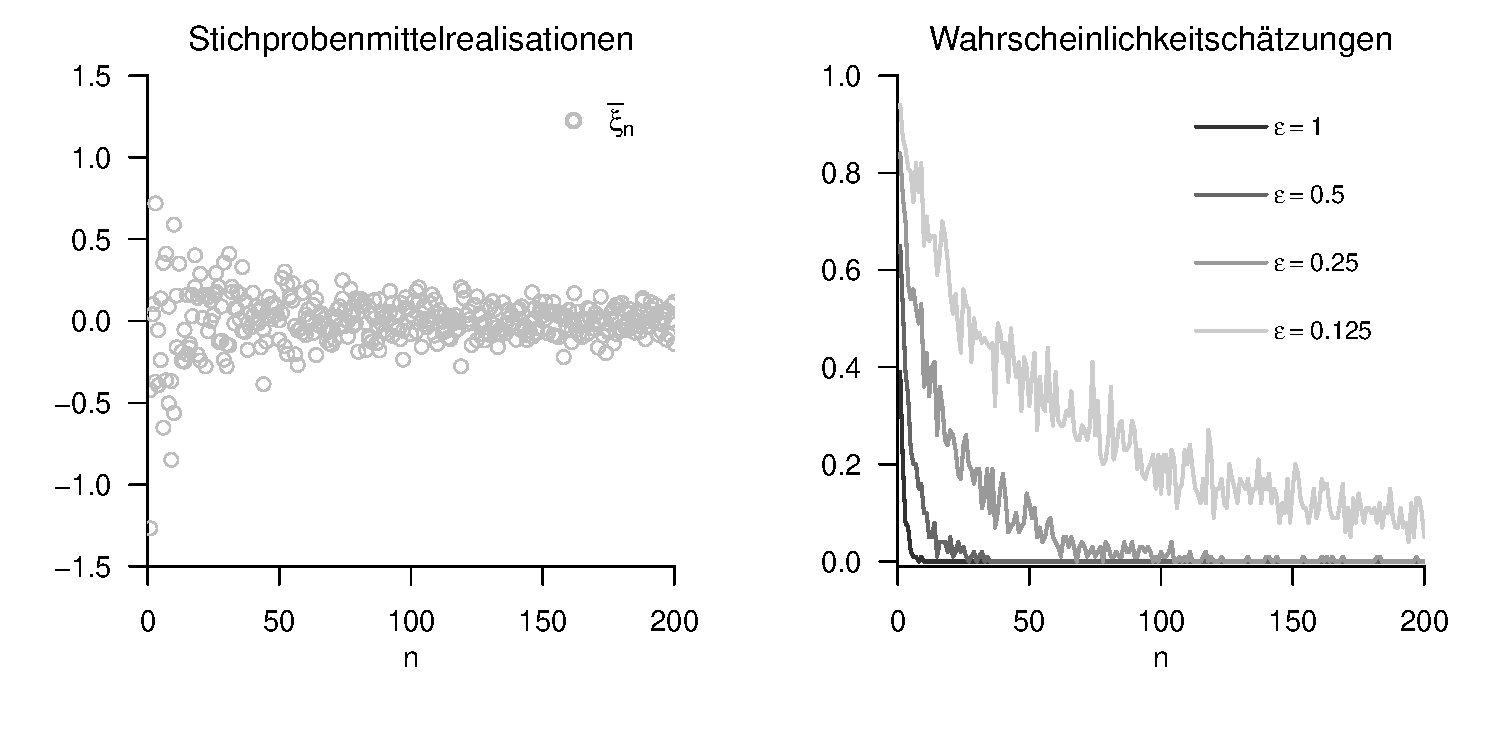
\includegraphics[width=0.95\linewidth]{7_Abbildungen/wtfi_7_schwaches_gesetz} \end{center}
\end{frame}

\begin{frame}{}
\protect\hypertarget{section-6}{}
\large
\vfill
\setstretch{2.5}

Wahrscheinlichkeitsungleichungen

Erwartungswertungleichungen

Gesetze der Großen Zahl

\textbf{Zentrale Grenzwertsätze}

Selbstkontrollfragen \vfill
\end{frame}

\begin{frame}{Zentrale Grenzwertsätze}
\protect\hypertarget{zentrale-grenzwertsuxe4tze}{}
Überblick \footnotesize

\begin{itemize}
\tightlist
\item
  \justifying Die Zentralen Grenzwertsätze besagen, dass die Summe von
  unabhängigen Zufallsvariablen mit Erwartungswert 0 asymptotisch, d.h.
  für unendlich viele Zufallsvariablen, normalverteilt mit
  Erwartungswertparameter 0 ist.
\item
  Modelliert man eine Messgröße \(y\) also als Summe eines
  deterministischen Einflusses \(\mu\) und der Summe \begin{equation}
  \varepsilon := \sum_{i=1}^n \xi_i
  \end{equation} einer Vielzahl von unabhängigen Zufallsvariablen
  \(\xi_i, i = 1,...,n\), welche unbekannte Störeinflüsse beschreiben,
  so ist für großes \(n\) die Annahme
  \begin{equation}\label{eq:stat_model}
  y = \mu + \varepsilon \mbox{ mit } \varepsilon \sim N(0,\sigma^2)
  \end{equation} also mathematisch gerechtfertigt. Wie wir später sehen
  werden, liegt die Annahme in Gleichung \eqref{eq:stat_model} vielen
  statischen Modellen zugrunde.
\item
  In der ``Lindenberg und Lévy'' Form des Zentralen Grenzwertsatzes
  werden unabhängig und identische Zufallsvariablen vorausgesetzt. In
  der ``Liapunov'' Form werden nur unabhängige Zufallsvariablen
  voraussetzt. Der Beweis der ``Lindenberg und Lévy'' Form ist einfacher
  als der Beweis der ``Liapunov'' Form. Wir verzichten hier abe rauf die
  Angabe von Beweisen.
\item
  In beiden Formulierungen des Zentralen Grenzwertsatzes die betrachtete
  Konvergenz von Zufallsvariablen die \emph{Konvergenz in Verteilung},
  welche wir zunächst einführen.
\end{itemize}
\end{frame}

\begin{frame}{Zentrale Grenzwertsätze}
\protect\hypertarget{zentrale-grenzwertsuxe4tze-1}{}
\footnotesize
\begin{definition}[Konvergenz in Verteilung]
\justifying
Eine Folge $\xi_1,\xi_2,...$ von Zufallsvariablen \textit{konvergiert in Verteilung 
gegen eine Zufallsvariable $\xi$}, wenn
\begin{equation}
\lim_{n \to \infty} P_{\xi_n}(x) = P_\xi(x).
\end{equation}
für alle $\xi$ an denen $P_\xi$ stetig ist.
Die Konvergenz in Verteilung von $\xi_1,\xi_2,...$ gegen $\xi$ wird geschrieben als
\begin{equation}
\xi_n\xrightarrow[n\to \infty]{\text{D}} \xi,
\end{equation}
Gilt $\xi_n\xrightarrow[n\to \infty]{\text{D}} \xi$, dann heißt die Verteilung von 
$\xi$ die \textit{asymptotische Verteilung der Folge $\xi_1,\xi_2,...$}.
\end{definition}
\footnotesize

Bemerkungen

\begin{itemize}
\tightlist
\item
  \(\xi\xrightarrow[n\to \infty]{\text{D}} \xi\) ist eine Aussage über
  die Konvergenz von KVFs.
\item
  Konvergenz in Wahrscheinlichkeit impliziert Konvergenz in Verteilung.
\end{itemize}
\end{frame}

\begin{frame}{Zentrale Grenzwertsätze}
\protect\hypertarget{zentrale-grenzwertsuxe4tze-2}{}
\footnotesize
\begin{theorem}[Zentraler Grenzwertsatz nach Lindenberg und Lévy]
\justifying
\normalfont
$\xi_1,...,\xi_n$ seien unabhängig und identisch verteilte Zufallsvariablen mit
\begin{equation}
\mathbb{E}(\xi_i) := \mu \mbox{ und }
\mathbb{V}(\xi_i) := \sigma^2 > 0
\mbox{ für alle } i = 1,....,n.
\end{equation}
Weiterhin sei $\zeta_n$ die Zufallsvariable definiert als
\begin{equation}
\zeta_n := \sqrt{n}\left(\frac{\bar{\xi}_n - \mu}{\sigma}\right).
\end{equation}
Dann gilt für alle $z \in \mathbb{R}$
\begin{equation}
\lim_{n \to \infty} P_{\zeta_n}(z) = \Phi(z),
\end{equation}
wobei $\Phi$ die kumulative Verteilungsfunktion der Standardnormalverteilung bezeichnet.
\end{theorem}

\footnotesize

Bemerkung

\begin{itemize}
\tightlist
\item
  Wir zeigen später, dass damit für \(n\to\infty\) asymptotisch auch
  gilt, dass \begin{equation}
  \sum_{i=1}^n \xi_i \sim N(n\mu, n\sigma^2)
  \mbox{ und }
  \bar{\xi}_n \sim N\left(\mu,\frac{\sigma^2}{n}\right).
  \end{equation}
\end{itemize}
\end{frame}

\begin{frame}{Zentrale Grenzwertsätze}
\protect\hypertarget{zentrale-grenzwertsuxe4tze-3}{}
\small

Beispiel (\(\xi_1,...,\xi_n \sim \chi^2(k)\))

\footnotesize

\begin{itemize}
\tightlist
\item
  Wir halten ohne Beweis fest, dass \(\mathbb{E}(\xi_i) = k\) und
  \(\mathbb{V}(\xi_i) = 2k\).
\item
  Wir betrachten das Szenario \(\xi_i \sim \chi(3)\) für
  \(i = 1,...,n\).
\item
  Die linken Abbildungen zeigen Histogrammschätzer der
  Wahrscheinlichkeitsdichte von \begin{equation}
  \zeta_n := \sqrt{n}\left(\frac{\bar{\xi}_n - \mu}{\sigma}\right)
  \end{equation} basierend auf 1000 Realisationen von \(\zeta_n\) für
  \(n = 2\) und \(n = 200\), sowie die WDF von \(N(0,1)\).
\item
  Die rechte Abbildung zeigt die entsprechenden (empirischen)
  kumulativen Verteilungsfunktionen.
\end{itemize}

\vspace{1mm}

\begin{center}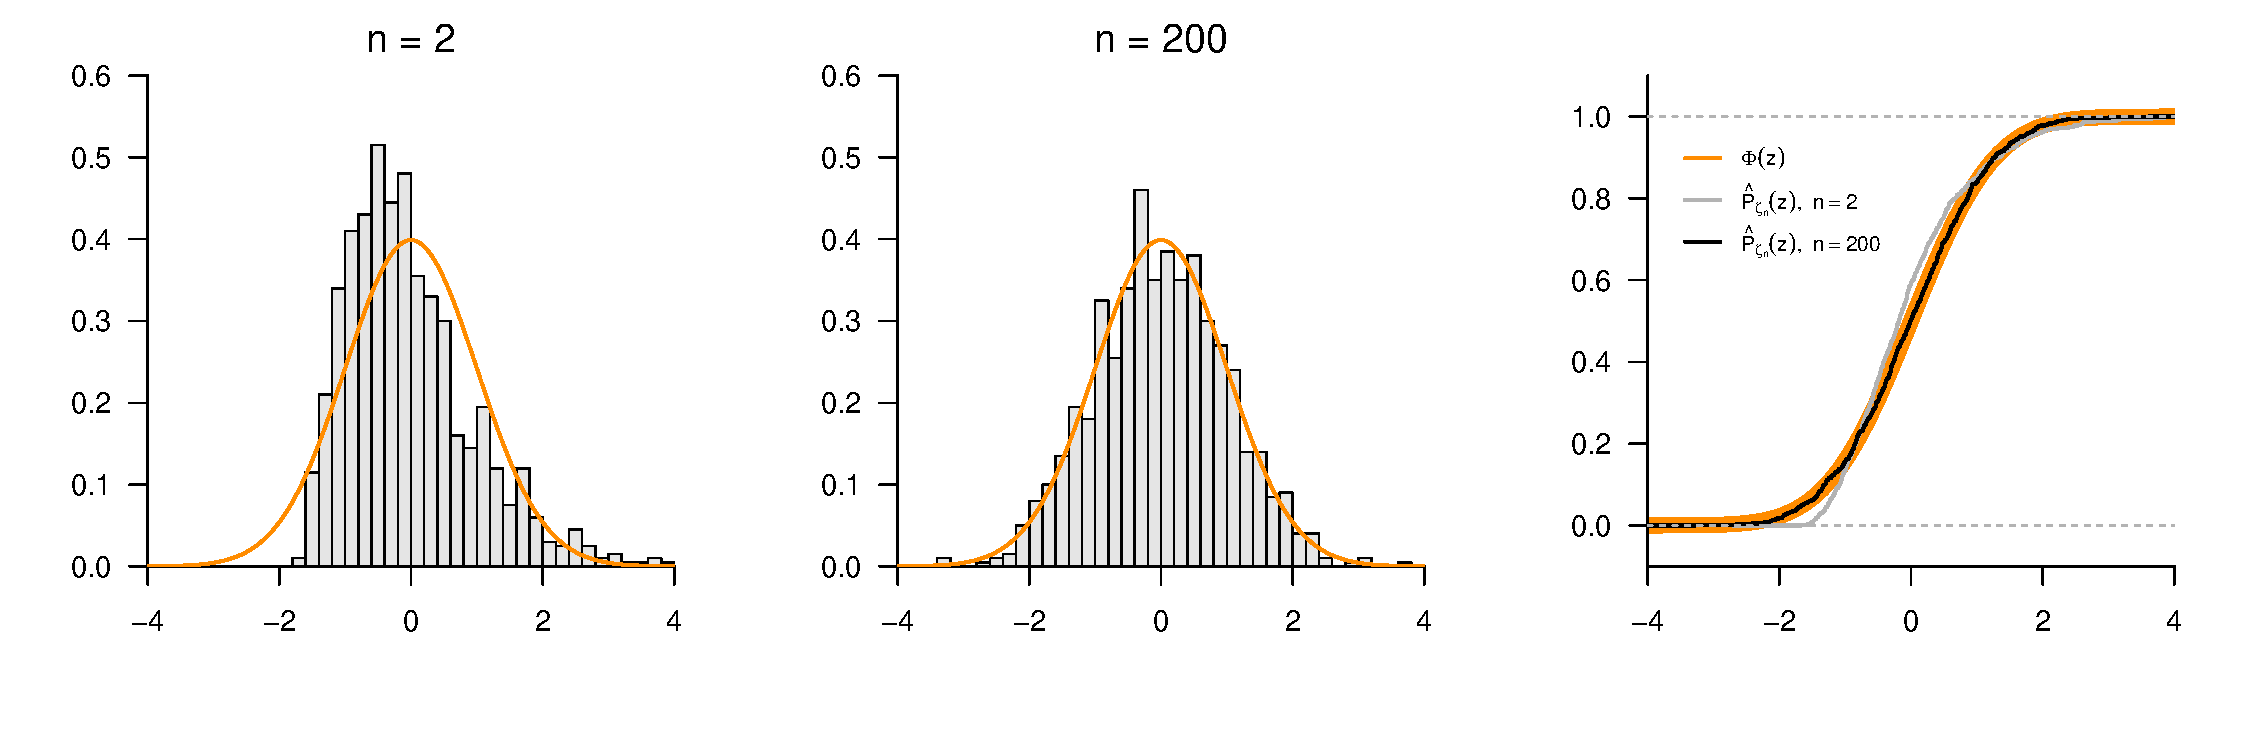
\includegraphics[width=0.95\linewidth]{7_Abbildungen/wtfi_7_lindenberg_levy} \end{center}
\end{frame}

\begin{frame}{Zentrale Grenzwertsätze}
\protect\hypertarget{zentrale-grenzwertsuxe4tze-4}{}
\footnotesize
\begin{theorem}[Zentraler Grenzwertsatz nach Liapounov]
\justifying
\normalfont
$\xi_1,...,\xi_n$ seien unabhängige aber nicht notwendigerweise identisch verteilten Zufallsvariablen mit
\begin{equation}
\mathbb{E}(\xi_i) := \mu_i \mbox{ und }
\mathbb{V}(\xi_i) := \sigma^2_i > 0
\mbox{ für alle } i = 1,....,n.
\end{equation}
Weiterhin sollen für $\xi_1,...,\xi_n$ folgend Eigenschaften gelten:
\begin{equation}
\mathbb{E}(|\xi_i - \mu_i|^3) < \infty \mbox{ und }
\lim_{n \to \infty} \frac{\sum_{i=1}^n \mathbb{E}\left(|\xi_i - \mu_i|^3\right)}{(\sum_{i=1}^n \sigma_i^2)^{3/2}} = 0.
\end{equation}
Dann gilt für die Zufallsvariable $\zeta_n$ definiert als
\begin{equation}
\zeta_n := \frac{\sum_{i=1}^n \xi_i - \sum_{i=1}^n \mu_i}{\sqrt{\sum_{i=1}^n \sigma_i^2}},
\end{equation}
für alle $z\in\mathbb{R}$, dass
\begin{equation}
\lim_{n \to \infty} P_{\zeta_n}(z) = \Phi(z),
\end{equation}
wobei $\Phi$ KVF der Standardnormalverteilung bezeichnet.
\end{theorem}

Bemerkungen

\begin{itemize}
\tightlist
\item
  Wir zeigen später, dass dann auch gilt, dass
  \(\sum_{i=1}^n \xi_i \sim N\left(\sum_{i=1}^n \mu_i, \sum_{i=1}^n \sigma_i^2\right)\).
\end{itemize}
\end{frame}

\begin{frame}{}
\protect\hypertarget{section-7}{}
\large
\vfill
\setstretch{2.5}

Wahrscheinlichkeitsungleichungen

Erwartungswertungleichungen

Gesetze der Großen Zahl

Zentrale Grenzwertsätze

\textbf{Selbstkontrollfragen} \vfill
\end{frame}

\begin{frame}{Selbstkontrollfragen}
\protect\hypertarget{selbstkontrollfragen}{}
\setstretch{1.7}
\small
\begin{enumerate}
\item Geben Sie die Markov Ungleichung wieder.
\item Geben Sie die Chebyshev Ungleichung wieder.
\item Geben Sie die Cauchy-Schwarz Ungleichung wieder.
\item Geben Sie die Korrelationsungleichung wieder.
\item Definieren Sie den Begriff der Konvergenz in Wahrscheinlichkeit.
\item Definieren Sie den Begriff der Konvergenz in Verteilung.
\item Geben Sie das Schwache Gesetz der Großen Zahl wieder.
\item Erläutern Sie den Zentralen Grenzwertsatz nach Lindenberg und Lévy.
\item Erläutern Sie den Zentralen Grenzwertsatz nach Liapunov.
\item Warum sind die Zentralen Grenzwertsätze für die statistische Modellbildung wichtig?
\end{enumerate}
\end{frame}

\begin{frame}{References}
\protect\hypertarget{references}{}
\footnotesize

\hypertarget{refs}{}
\begin{CSLReferences}{1}{0}
\leavevmode\vadjust pre{\hypertarget{ref-degroot_probability_2012}{}}%
DeGroot, Morris H., and Mark J. Schervish. 2012. \emph{Probability and
Statistics}. 4th ed. {Boston}: {Addison-Wesley}.

\leavevmode\vadjust pre{\hypertarget{ref-georgii_stochastik_2009}{}}%
Georgii, Hans-Otto. 2009. \emph{{Stochastik: Einführung in die
Wahrscheinlichkeitstheorie und Statistik}}. 4., überarb. und erw. Aufl.
{De-Gruyter-Lehrbuch}. {Berlin}: {de Gruyter}.

\end{CSLReferences}
\end{frame}

\end{document}
